\section{Anwendersicht}
Für die Anwendersicht wurden zwei Applikationen erstellt. Zum einen eine Mobile Applikation und zum anderen eine Web Applikation. Die Mobile Applikation wurde für das Betriebssystem Android in AndroidStudio entwickelt. Die Web Applikation wurde mit Hilfe eines Bootstrap Templates erstellt. Beide Applikationen verwenden die Bibliothek Paho um mit der MOM zu Interagieren.  
\subsection{Android-App}
Die Android Applikation soll eine Wetter Applikation sein, dafür soll sie verschiedene Wetterdaten anzeigen können. Dazu wurde zu beginn des Projektes festgelegt, welche Daten anzeigt werden sollen. Diese können in zwei Kategorien unterschieden werden. Zum einen das \textbf{Tageswetter} und zum anderen die \textbf{Wochenvorhersage}. Unter das Tageswetter fallen die folgenden Punkte: 
\begin{itemize}
\item das Tageswetter als großes Icon
\item die momentane Temperatur in $^\circ$C
\item das genaues Wetter in Wörtern
\item der Standort
\item das Datum mit Uhrzeit
\item die Windgeschwindigkeit in km/h
\item die Windrichtung mit Hilfe einer grafischen Anzeige
\item die Regenwahrscheinlichkeit in \%
\end{itemize}  
Bei der Wettervorhersage für eine Woche ergeben sich nachfolgende Punkte
\begin{itemize}
\item die Wochentage ab dem Nachfolgetag des Tageswetters
\item ein kleines Wettericon
\item die Tagesmaximaltemperatur in $^\circ$C mit der Schriftfarbe rot
\item die Tagesminimaltemperatur in $^\circ$C mit der Schriftfarbe blau
\item ein Diagramm das die Maximal- und Minimaltemperaturen veranschaulicht
\end{itemize}  
Des Weiteren sollte es eine Auswahlmöglichkeit geben zwischen der Automatischen Standortbestimmung mittels GPS und der Eingabe einer Postleitzahl um den Standort festzulegen.
\begin{figure}[htbp]
	\centering
	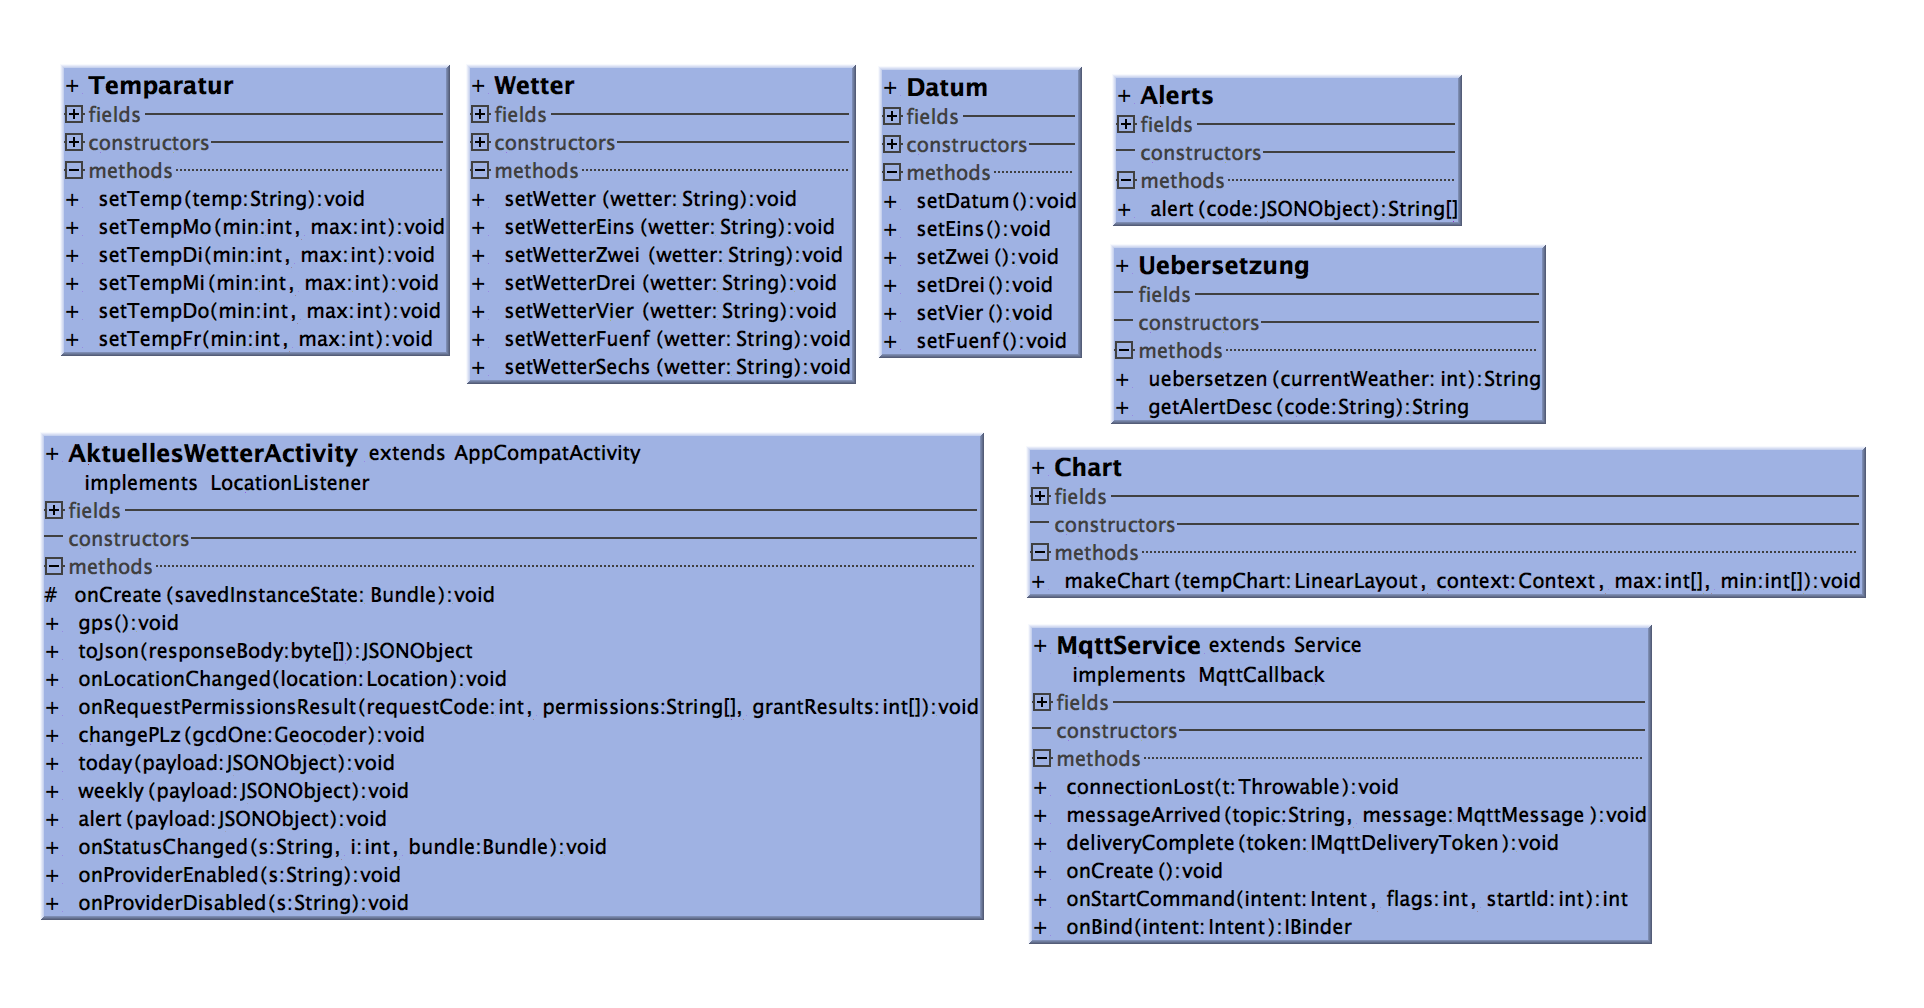
\includegraphics[width=1.0\textwidth]{Bilder/AndroidUML.png}
	\caption{Klassendiagramm der Android-Applikation}
	\label{img:AndroidUMLDiagramm}
\end{figure} 
Die Applikation wurde in Androidstudio in der Sprache Java und XML geschrieben. 
Aufgebaut ist die Applikation über 8 Klassen wie in  Abb. \ref{img:AndroidUMLDiagramm} zusehen ist. Die Klasse \textbf{AktuellesWetterActivity} fungiert dabei als Main-Class.
Die Klasse \textbf{MqttService} ist ein Android Service. Als einen Android Service bezeichnet man einen Prozess der nebenläufig zum Hauptprozess läuft. Dieser Service ist für die Verbindung zur MOM notwendig und wird später im Unterkapitel \ref{subsubsec:MqttService} näher erläutert.
Die weiteren Klassen sind Hilfsklassen zur Verarbeitung der, durch die MoM bereitgestellten Daten.
Beispielsweise übersetzt die Klasse \textbf{Uebersetzung} die verschiedenen Wettercodes in, für den Anwender lesbare, Wetterbezeichnungen. Dies geschieht mit Hilfe einer einfachen Switch-Case-Anweisung, wie exemplarisch in Abb. \ref{img:Case-Uebersetzung} zu sehen.
  \begin{lstlisting}
 switch (code) {
            case "H1": {
                return "Starke Luftdruckschwankungen, nehmen Sie Ihre Medizin falls benoetigt";
            }
            case "H2": {
                return "Temperaturen ueber 25 $^\circ$C, nehmen Sie Ihre Medizin falls benoetigt";
            }
            case "S1": {
                return "Ideales Badewetter";
            }
            case "W1": {
                return "Achtung, Frostgefahr";
            }
            case "W2": {
                return "Achtung, sehr niedrige Temperaturen. Ziehen Sie sich warm an.";
            }
            case "W3": {
                return "Achtung, schwere Schneefaelle.";
            }
            case "T1": {
                return "Luftfeuchtigkeit ueber 90%";
            }
        }
	\label{img:Case-Uebersetzung}
\end{lstlisting} 

Bei beginn der Applikation soll, wie in den Anforderungen beschrieben, die Position automatisch durch GPS ermittelt werden. Dazu wurde das von Android bereitgestellte Interface LocationListener verwendet. Dazu müssen die Methoden onLocationChanged(), onProviderDisabled(), onProviderEnabled() und onStatusChanged() implementiert werden. 
Die wichtigste Methode dabei ist die onLocationChanged(). Diese liefert jedes Mal wenn sich die Position des Smartphones verändert die neue Position zurück. 
Um nun das Interface LocationListener zu verwenden, ist es notwendig sich den Location Service bei den SystemServices zu holen. Dies geschieht über folgende Codezeile:
  \begin{lstlisting}
   LocationManager locationManager = (LocationManager) getSystemService(Context.LOCATION_SERVICE);
  \end{lstlisting}
  Des Weiteren ist es ab Android Version 6.0 (API level 23)notwendig dem Anwender die Möglichkeit zugeben, die Standortbestimmung mittels GPS zu verweigern. Dafür muss eine Permissions Abfrage gemacht werden, welche von Android fertig bereitgestellt und in den Code eingebaut werden kann. Wenn das geschehen ist, kann über das Objekt locationManager die Methode requestLocationUpdates(String provider,long minTime, float minDistance, LocationListener listener) mit den Parametern: 
    \begin{itemize}
\item provider = "gps"
\item minTime = 10000 (Millisekunden)(dieser Wert ist für die App nicht so wichtig, da die Aktualisierung nur beim Start und auf Knopfdruck benötigt wird)
\item minDistance = 50 (in Meter)(dieser Wert ist für diese App nicht so wichtig, da die Genauigkeit der Position eine untergeordnete Rolle spielt)
\item listener = this (Klasse die das Interface LocationListener implementiert)
\end{itemize}  
aufrufen. Nachdem diese Methode mit den Settings des LocationManagers ausgeführt wurde, kann die Methode getLastKnownLocation("gps") der Klasse LocationManager aufgerufen werden. Diese Methode liefert ein Objekt der Klasse Location zurück. Dieses Location Objekt beinhaltet die Positionsdaten. Um nun von den Positionsdaten auf die benötigten Angaben wie Stadtname und Postleitzahl (PLZ) zukommen, wird ein Objekt der Klasse Geocoder benötigt. Die Klasse Geocoder ist ebenfalls Bestandteil der Android Location Library. Durch diese Klasse können die Längen- und Breitengrad Daten des Location Objektes in Stadtnamen und PLZ umgewandelt werden.
Liegen diese Daten vor kann der Stadtname auf der App angezeigt werden und der Android Service MqttService mit dem Übergabeparameter PLZ über folgenden Code 
 \begin{lstlisting}
private Intent serv = new Intent(this, MqttService.class);
serv.putExtra("plz", plz); 
startService(serv);
  \end{lstlisting}
gestartet werden.
\subsubsection{Mqtt Service}
\label{subsubsec:MqttService}
Der MqttService ist das Herzstück der Android Applikation in diesem Service wird die Verbindung zur MOM hergestellt und die Daten die diese liefert empfangen.
Mit dem Open Source Projekt Paho wurde eine Verbindung zu der in Kapitel \ref{rabbitmq} vorgestellten MOM realisiert. Dafür wurde die für Android spezifische Library über Grovy importiert. Durch diesen Import ist es möglich einen Android-Client zu erstellen. Dafür wurde das Interface MqttCallback implementiert. Zu diesem Interface gehören die Methoden: 
 \begin{itemize}
\item connectionLost(Throwable t):
\\Diese Methode hat den Zweck, wenn während des Betriebs der Applikation die Verbindung zur MOM verloren geht, diese wieder aufzubauen.
\item messageArrived(String topic, MqttMessage message):
\\In dieser Methode kommen die Messages der Abonnierten Topics als Byte Arrays und das dazugehörige Topic als String, zur Unterscheidung der Messages an.
\item deliveryComplete(IMqttDeliveryToken token):
\\Wird aufgerufen, wenn die Zustellung für eine Nachricht abgeschlossen ist und alle Bestätigungen eingegangen sind.
\end{itemize}
Wie im vorherigen Kapitel erwähnt wird der Service mit dem Parameter PLZ gestartet, dazu wird die Methode onStartCommand verwendet, diese besitzt als Aufrufparameter ein Intentobjekt, diesem wurde in der AktuellesWetterActivity ein "Extra" mit dem Key plz übergeben. Mit Hilfe dieses Keys kann der Übergebene Wert ausgelesen werden. Um nun eine Verbindung mit der MOM aufzubauen, werden vier Angaben benötigt. Diese sind zum einen die tcp-url und der Port der MOM. Zum anderen für die Authentifizierung bei der MOM einen Usernamen und ein Passwort. Der Username und das Passwort werden einem Paho ConnectionOption Objekt übergeben. Dabei wird das Passwort mittels eines Char-Arrays übergeben. Dieses ConnectionOption Objekt wird wiederum zusammen mit der Url, dem Port und einer Client-Id (diese wird automatisch erzeugt) an das eigentlichen Client Objekt übergeben. Dieses Client Objekt besitzt die Methode connect in dieser wird das Interface IMqttActionListener mit den Methoden onSuccess und onFailure aufgerufen. In der Methode onSuccess werden nun 3 Topics der MOM abonniert. Diese 3 Topics sind:
\begin{itemize}
\item plz/today/CEP:
\\ Liefert ein JSON Objekt mit dem Tages aktuellen Wetter für die Postleitzahl.
\item plz/weekly/CEP:
\\ Liefert ein JSON Array mit dem Wochenwettervorhersagen für die Postleitzahl.
\item plz/alert:
\\ Liefert ein JSON Objekt falls es eine Wetterwarnung für die Postleitzahl gibt.
\end{itemize}
Im Falle das eine Nachricht der MOM eintrifft wird, wird die weiter oben im Kapitel erwähnte Methode messageArrived aufgerufen.
Mit Hilfe eines BroadcastReceivers und einem weiteren Intentobjekts wird diese Nachricht an die AktuellesWetterActivity Klasse übergeben.
\subsubsection{Broadcast Receiver}
\label{subsubsec:BroadcastReceiver}
Ein Broadcast Receiver ist neben einem Activity und einem Service, eine weitere wichtige Komponente bei Android. Mit Hilfe eines BroadcastReceiver ist es möglich Nachrichten mit Hilfe eines Intentobjektes über Prozessgrenzen hinaus zu versenden. Ein BroadcastReceiver hat nur eine solange Lebensdauer wie es benötigt die erhaltene Nachricht zu bearbeiten. Ist diese Nachricht verarbeitet wird die Instanz des BroadcastReceivers beendet. Dies hat den Vorteil das der Akkuverbrauch des Smartphones gesenkt wird. Um einen BroadcastReceivers verwenden zu können muss dieser beim System mit einem Namen registriert werden, dies zeigt die nachfolgende Codezeile:
\begin{lstlisting}
 LocalBroadcastManager.getInstance(this).registerReceiver(broadcastReceiver, new IntentFilter("NOW"));
  \end{lstlisting}
Dieser BroadcastReceivers wurde mit dem Namen "NOW" registriert.
Innerhalb dieses Receivers wird nun die Ausgabe der Daten, die von der MOM gesendet wurden, geregelt. Dazu wird über das Topic entschieden wie mit der angekommenen Message verfahren wird (siehe nachfolgendes Codefragment).
\begin{lstlisting}
public void onReceive(Context context, Intent intent) {
            byte[] mes = intent.getByteArrayExtra("Message");
            Log.e("onReceive: ", new String(mes));
            if (new String(mes).contains("hallo")) {
            } else {
                JSONObject payload = toJson(mes);
                String topic = intent.getStringExtra("Topic");
                if (topic.contains("today")) {
                    today(payload);
                } else {
                    if (topic.contains("weekly")) {
                        weekly(payload);
                    } else if (topic.contains("alert")) {
                        alert(payload);
                    }
                }
            }
        }
  \end{lstlisting}
  
  Um nun das in den Anforderungen gewünschte Diagramm zu erzeugen gibt es die Klasse Chart. Diese erzeugt mit Hilfe der in Weekly enthaltenen Minimum- und Maximumtemperaturen für die einzelnen Tagen ein Liniendiagramm. Dazu wurde die free Library aChartengine verwendet.
Die nachfolgende Abb. \ref{img:AndroidApplikation} zeigt die fertige Applikation mit dem Tageswetter und der Wochenvorhersage.

\begin{figure}
    \subfigure{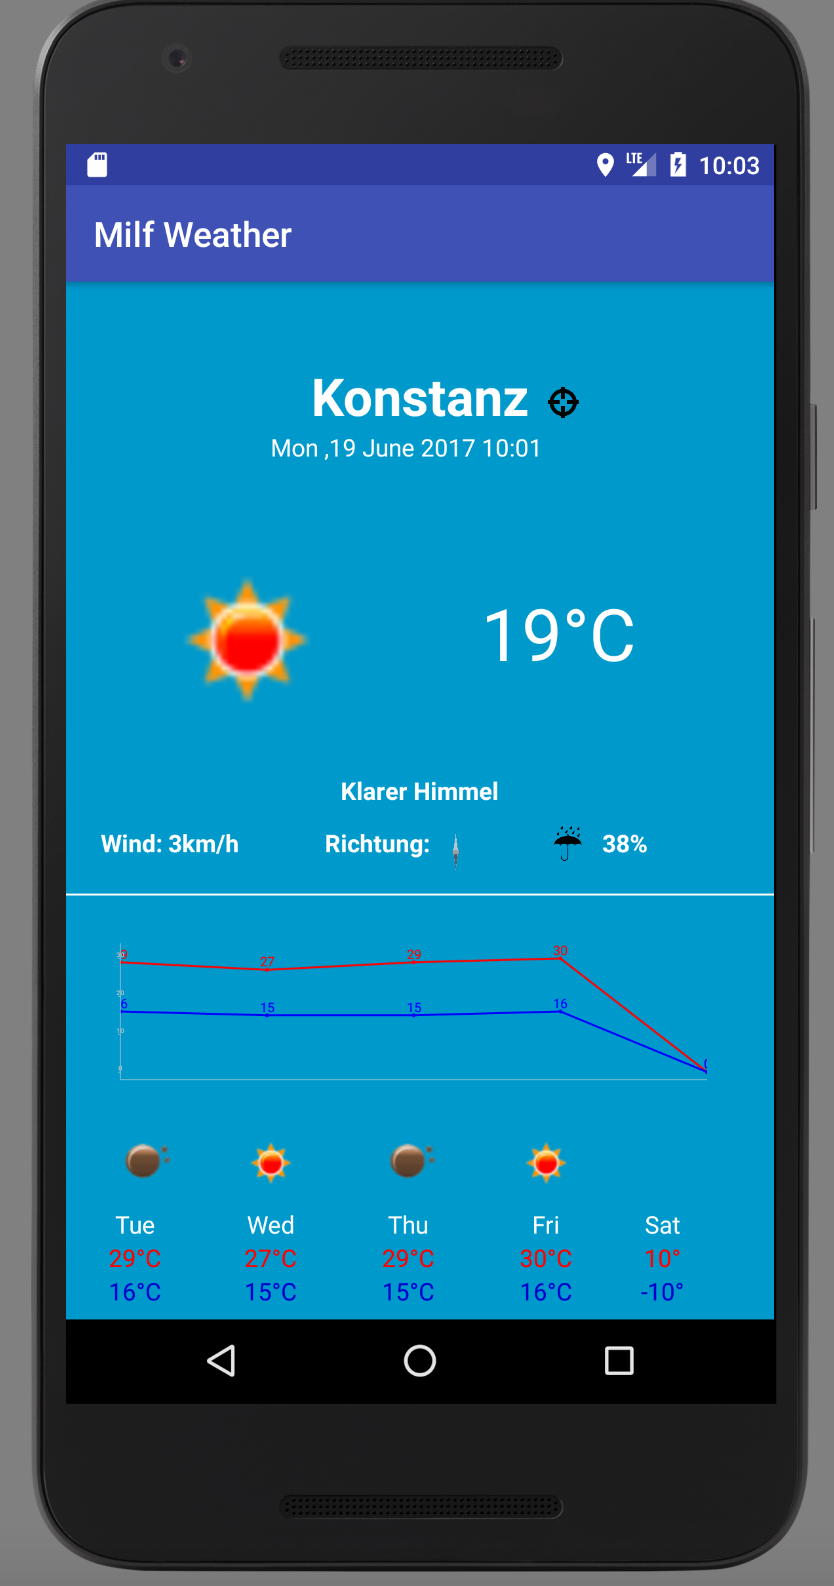
\includegraphics[width=0.5\textwidth]{Bilder/AndroidApp.png}}
    \subfigure{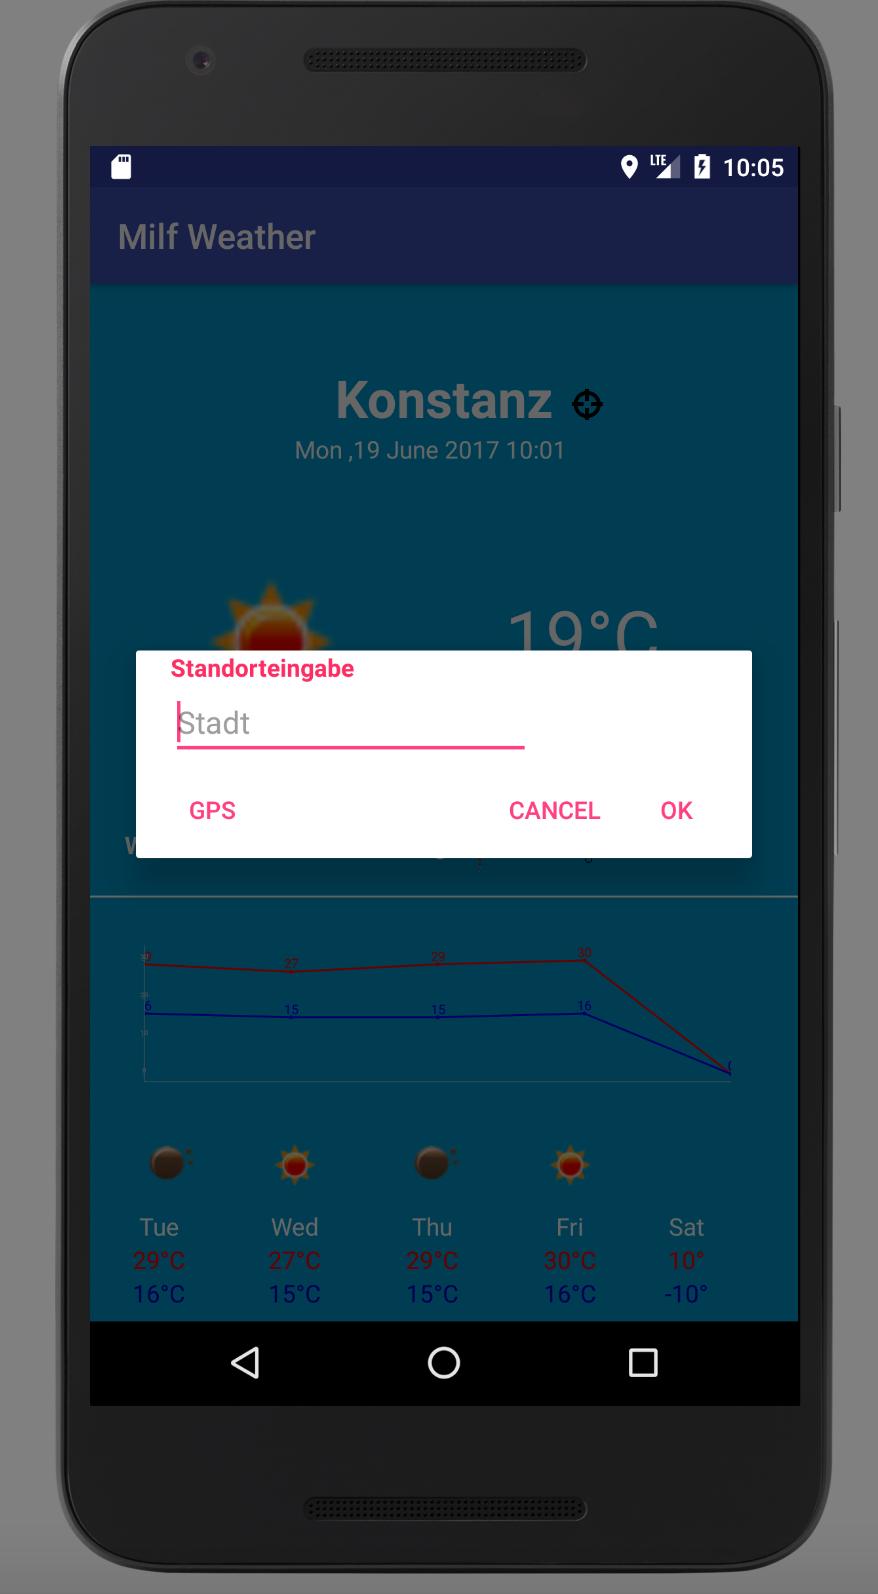
\includegraphics[width=0.5\textwidth]{Bilder/AndroidAppPLZ.png}}
\caption{Android-Applikation}
\label{img:AndroidApplikation}
\end{figure}


\subsection{Web-Client} \label{Web-Client}
Der Web-Client stellt dem Endnutzer eine Darstellung der Wetterdaten zur Verfügung. Die angezeigten Daten gleichen denen der Android-App, die Darstellungsform ist jedoch für größere Bildschirme optimiert. 
\subsubsection{Layout}
Das Layout der Applikation baut auf ein Template von Bootstrap auf und ist untergliedert in die Navigationsleiste am oberen Rand, einen sogenannten Jumbotron Container für das aktuelle Wetter, einem Block für die Vorhersage und schlussendlich einen Footer. 
\begin{figure}[htbp]
	\centering
	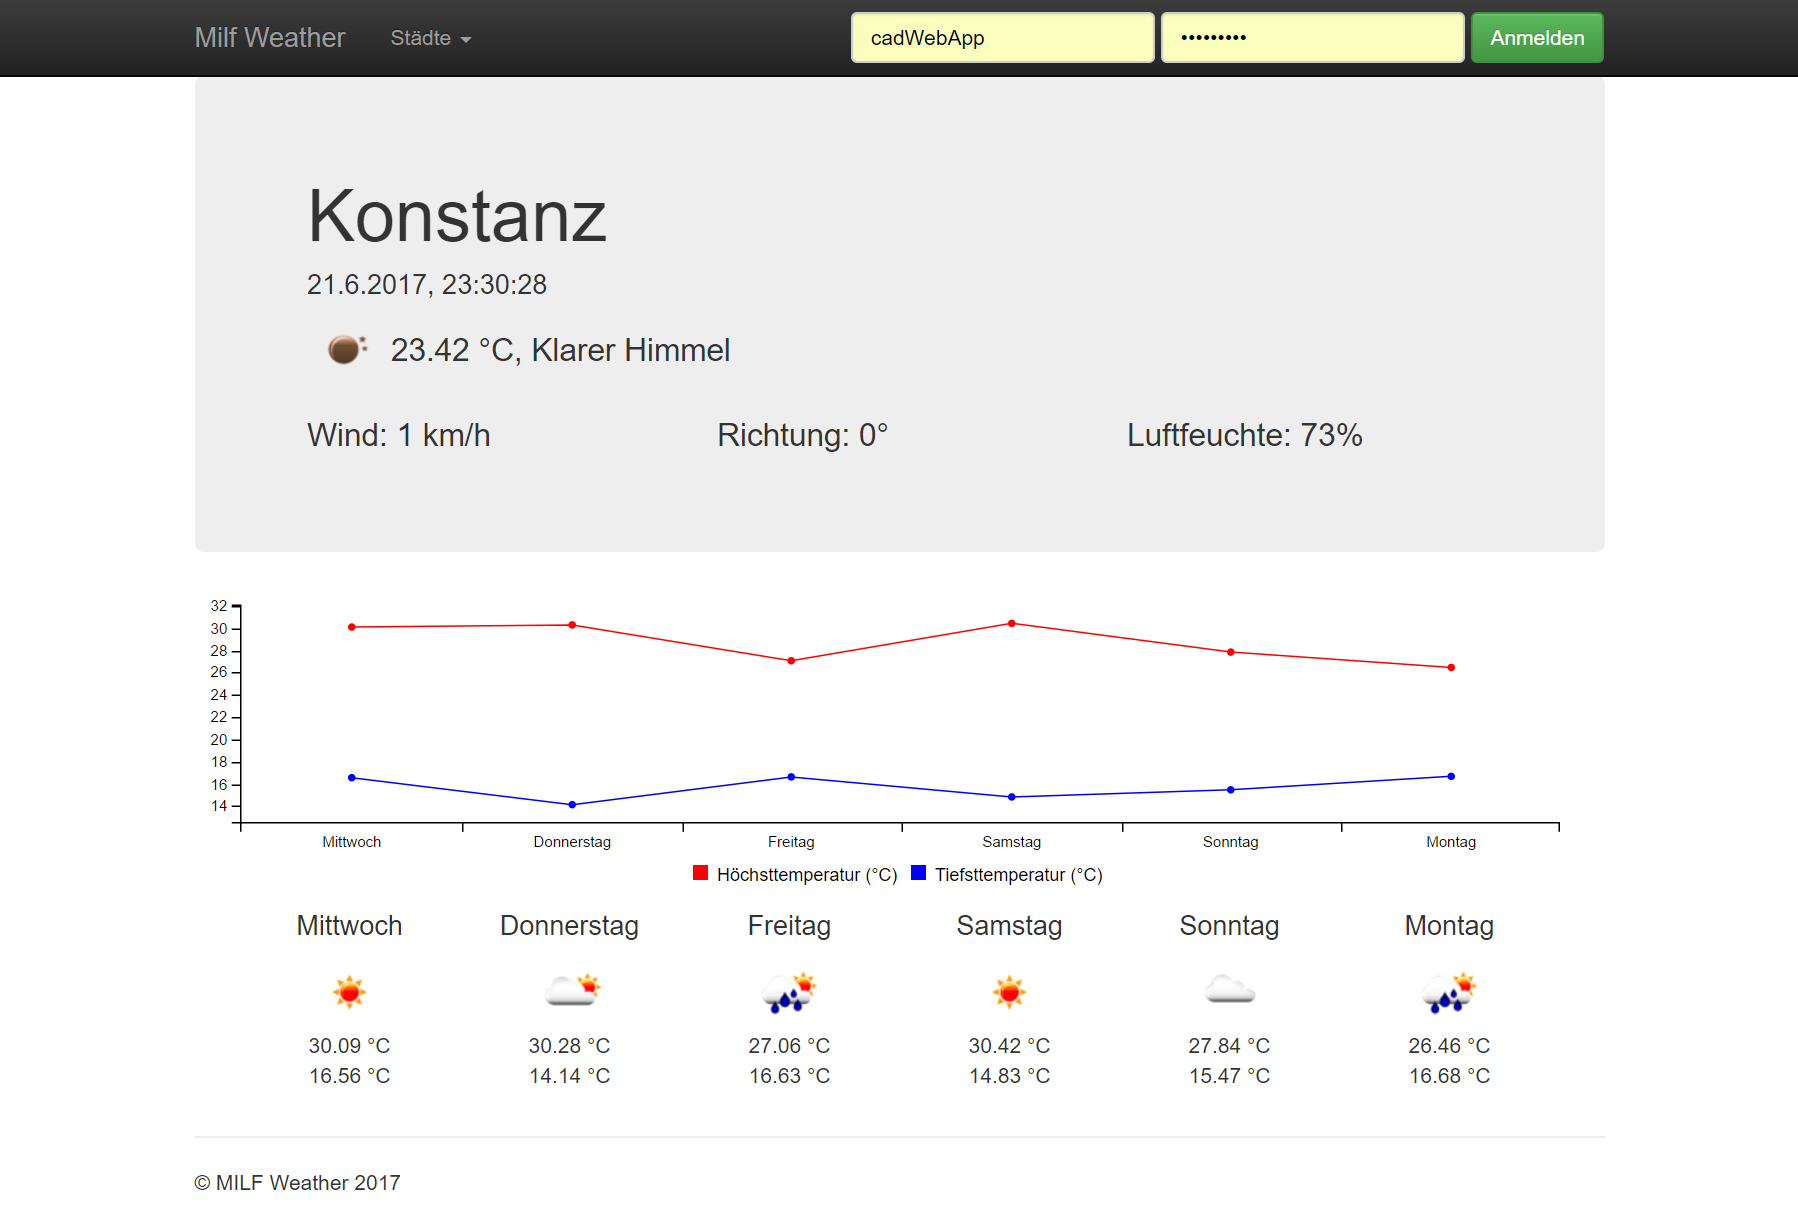
\includegraphics[width=1.0\textwidth]{Bilder/Web-Client.png}
	\caption{Web-Client}
	\label{img:webclient}
\end{figure}
Die Navigationsleiste enthält neben dem Seitennamen ein Dropdown-Menü, über welches die Auswahl der Stadt erfolgt, und ein Login Formular mit Eingabefeldern für den Benutzernamen und das Passwort sowie einen Button. Reicht der Platz zur Darstellung nicht aus, werden die Stadtauswahl und Loginmaske durch einen Button ersetzt, über den sich die Navigationsleiste ausfahren lässt um dann die Funktionen dort anzuzeigen.
Unterhalb der Navigationsleiste schließt ein farblich abgetrennter Bereich an, in dem prominent das aktuelle Wetter, der gewählte Ort sowie Datum und Uhrzeit dargestellt werden. Die Wetterdarstellung umfasst eine graphische Repräsentation in Form eines Icons, die aktuelle Temperatur in Grad Celsius, eine textuelle Beschreibung des Wetters sowie die Windgeschwindigkeit in km/h, die Windrichtung und die Luftfeuchtigkeit.
Anschließend wird die prognostizierte Höchst- und Tiefsttemperatur über den Wochentagen in einem Diagramm dargestellt und direkt darunter wird eine Wetterdarstellung in Form eines Icons sowie die Höchst- und Tiefsttemperatur textuell dargestellt.
Am Schluss der Webseite kommt ein Footer, der Platz bietet für rechtliche Informationen.

Technische Umsetzung
Auf technischer Seite nutzt die Webapplikation die Sprachen PHP, JavaScript, HTML und css. PHP wird ausschließlich verwendet um die Variablen, welche für die Verbindung zu Message Oriented Middleware benötigt werden, aus den beim Serverhost konfigurierbaren Umgebungsvariablen auszulesen, wie in Abb.\ref{img:Einbindung PATH-Variablen} zu sehen.
\begin{lstlisting} 
<script type="text/javascript">
  momAddress = "<?php echo getenv("momAddress"); ?>";
  momPort = "<?php echo getenv("momPort"); ?>";
  tenant = "<?php echo getenv("tenant"); ?>";
  topicToday = "<?php echo getenv("topicToday"); ?>";
  topicWeek = "<?php echo getenv("topicWeek"); ?>";
  topicAlert = "<?php echo getenv("topicAlert"); ?>";
</script>
\label{img:Einbindung PATH-Variablen}
\end{lstlisting}
Die Verbindung zur MOM wird clientseitig über die JavaScript Bibliothek Paho aufgebaut. Paho ist ein Projekt der Eclipse Foundation - bekannt vor allem für die gleichnamige IDE - mit dem Ziel Internet of Things Applikationen die Implementierung des MQTT Protokolls zu vereinfachen. Paho ist für eine ganze Reihe von Sprachen verfügbar, darunter Java, Python, C, C++ und dem hier verwendeten JavaScript. Der Funktionsumfang unterscheidet sich jedoch und so unterstützt die JavaScript Version nicht das Standard MQTT Protokoll, sondern nur eine angepasste Version für WebSockets. Für RabbitMQ lässt sich die Unterstützung von WebSockets über das RabbitMQ Web MQTT Plugin hinzufügen. Dies ermöglicht eine direkte Verbindung zwischen dem Browser des Nutzers und der MOM, ohne weitere Interaktion mit dem Webserver.
In Kombination mit der Umsetzung als Single Page Application bedeutet dies eine minimale Belastung des Webservers und erlaubt somit eine große Anzahl Nutzer pro Server. Bei Herokus kostenlosem Hostingmodell, welches nur 512 MB RAM und einen Worker bereitstellt waren so bereits in Tests über einen Zeitraum von einer Minute 1500 Aufrufe der Seite pro Sekunde möglich (vgl. Abb.\ref{img:testsettings} und \ref{img:testresults}.
\begin{figure}[htbp]
	\centering
	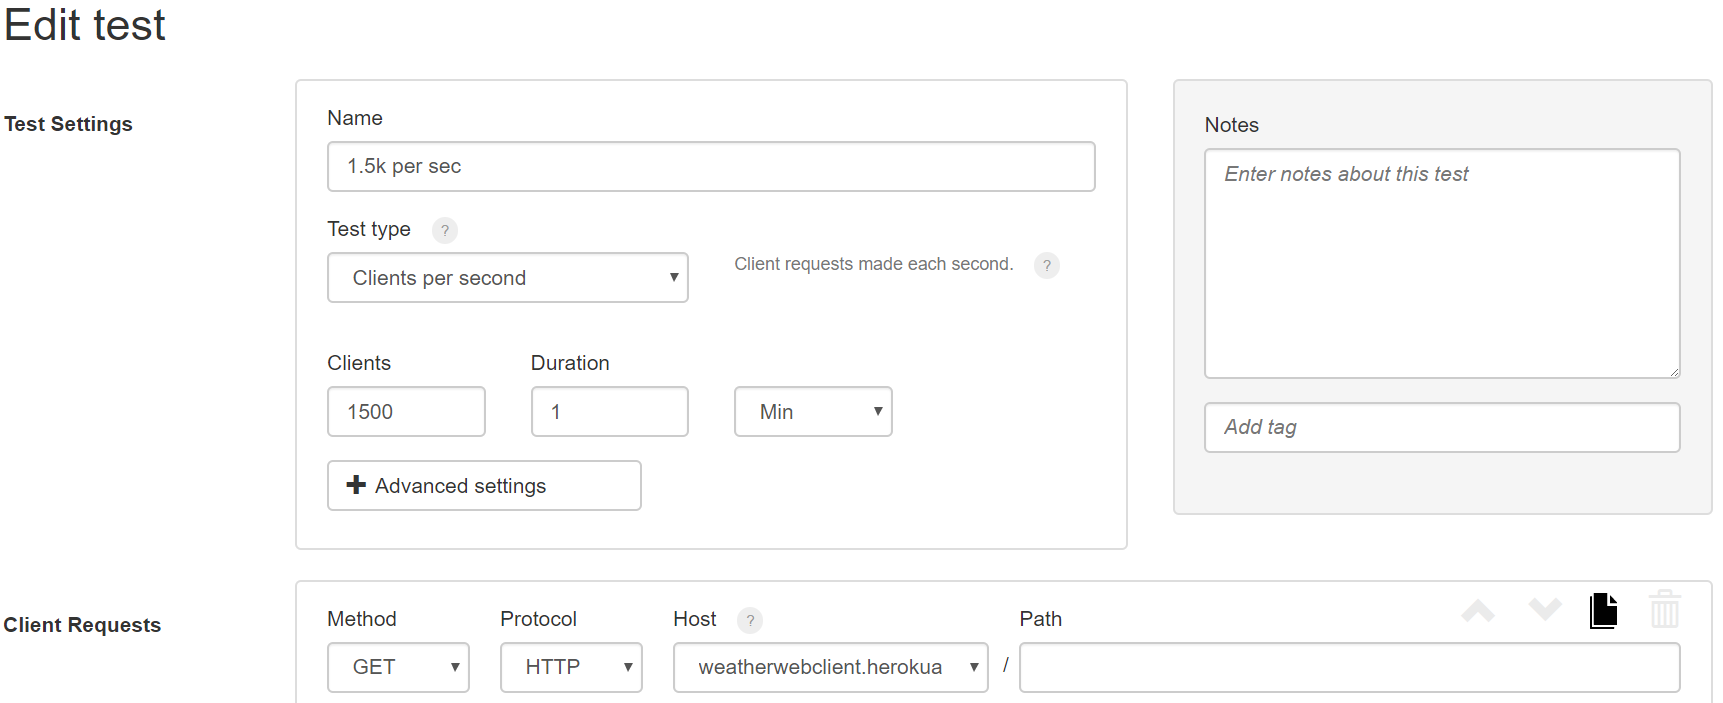
\includegraphics[width=1.0\textwidth]{Bilder/Web-TestSettings.png}
	\caption{Testeinstellungen}
	\label{img:testsettings}
\end{figure}
\begin{figure}[htbp]
	\centering
	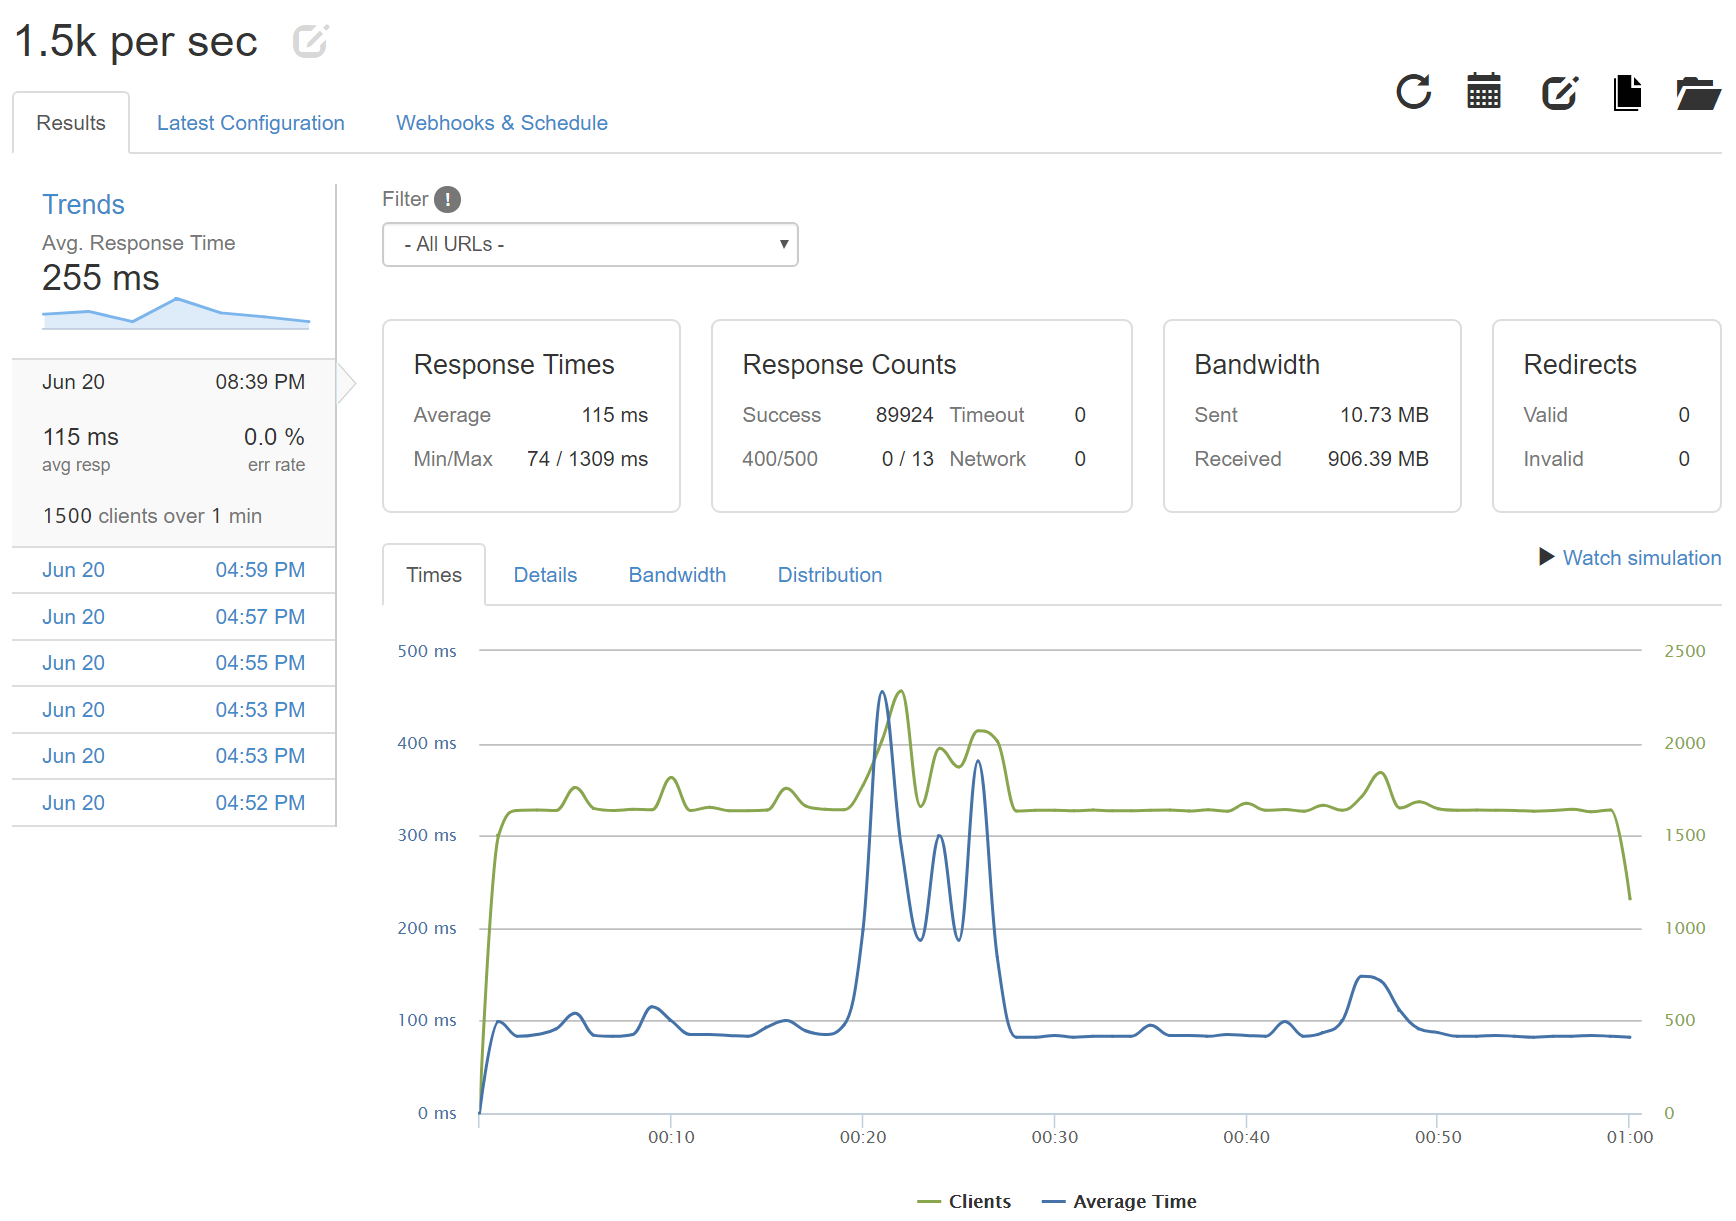
\includegraphics[width=1.0\textwidth]{Bilder/Web-TestErgebnisse.png}
	\caption{Testeinstellungen}
	\label{img:testresults}
\end{figure}
. Getestet wurde dies über den cloudbasierten Lasttest der SendGrid Labs, welcher unter der Webseite www.loader.io verfügbar ist und in einem AWS Rechenzentrum an der amerikanischen Ostküste läuft. 
Kommt der Benutzer auf die Webseite kann er eine Stadt wählen und sich einloggen. Der Login startet im JavaScript Code die Funktion connect und löst somit einen Verbindungsversuch zur MOM aus. Wurde beim Nutzername der Tenant nicht mit angegeben wird automatisch der Default-Tenant verwendet. Bei erfolgreicher Verbindung wird der Callback onConnect aufgerufen, der die Topics für das aktuelle Wetter, die Vorhersage und die Wetterwarnungen des gewählten Ortes abonniert. Geht zu einem Topic eine neue Nachricht ein wird diese in der Funktion onMessageArrived behandelt. Hierbei wird unterschieden zu welchem Topic die Nachricht gehört und im Fall des aktuellen Wetters oder der Vorhersage auch, ob die Nachricht neue Informationen enthält. Ist dies nicht der Fall wird die Nachricht nicht weiter behandelt, da dies an den dargestellten Informationen nichts ändern würde. Unterscheidet sich die Nachricht zur vorherigen wird die Nachricht dekodiert und die neuen Informationen werden mit Hilfe von jQuery-Funktionen in der HTML-Darstellung eingebunden, wie nachfolgend zu sehen ist. 
\begin{lstlisting} 
switch (message.destinationName) {
  case topicToday:
    //console.log("today: ", message.payloadString);
    todayData = message.payloadString;
    if (todayData != todayDataLast) {
      todayDataLast = todayData;
      var data = JSON.parse(todayData);
      $("#nowImage").attr("src", "img/" + data.weatherIcon + ".png");
      $("#nowTemp").text(data.temperature);
      $("#nowDescription").text(getWeatherDesc(data.currentWeatherId));
      $("#nowWindSpeed").text(data.windspeed);
      $("#nowWindDirection").text(data.windDeg);
      $("#nowHumidity").text(data.humidity);
      ...      
    }
    ...
}
\label{img:Verarbeiten-des-Topics-today}
\end{lstlisting}


Zur Generierung des Graphen (vgl. \ref{img:renderGraph}) wird die Bibliothek c3.js benutzt, welche wiederum intern d3.js verwendet, jedoch die Erstellung von Diagrammen mit weniger und einfacherem Quellcode ermöglicht als bei d3.js nötig wäre. Die erzeugten Graphen passen sich an die Anzahl, Minimal- und Maximalwerte der zu visualisierenden Daten an und skalieren mit der Bildschirmgröße. Die Konfiguration des Diagramms erfolgt über die Funktion generateGraph. Hier wird unter „bindto“ der css-selector angegeben, in dem der Graph erzeugt werden soll. Die Größe wird unter „size“ auf eine Höhe von 200 Pixeln begrenzt, unter „axis.x“ wird die Beschriftung entlang der X-Achse definiert. Entlang der y-Achse passt sich die Skala automatisch an die unter „data.columns“ eingetragenen Daten an. Die Datenpaare werden mit Höchst- bzw. Tiefsttemperatur benannt und farblich rot bzw. blau definiert. Über den Punkt padding wird der linke sowie rechte Abstand zum Container festgelegt. Hier muss genügend Platz für die Beschriftung links sein, da die Außenpunkte für die Darstellung der Start- bzw. Endpunkt der X-Achse ist. Um die schriftliche Vorhersage ausgerichtet unter dem Graphen darzustellen muss im css für diese der gleiche Abstand, jedoch als Margin, festgelegt werden.

\begin{lstlisting} 
// renders the graph
function generateGraph(data) {
  c3.generate({
    bindto: "#chart",
    size: {
      height: 200
    },
    data: {
      columns: [
        ["Hoechsttemperatur (Grad C)",
          data.days[0].temperatureMax, data.days[1].temperatureMax, data.days[2].temperatureMax,
          data.days[3].temperatureMax, data.days[4].temperatureMax, data.days[5].temperatureMax],
        ["Tiefsttemperatur (Grad C)",
          data.days[0].temperatureMin, data.days[1].temperatureMin, data.days[2].temperatureMin,
          data.days[3].temperatureMin, data.days[4].temperatureMin, data.days[5].temperatureMin]
      ],
      colors: {
        "Hoechsttemperatur (Grad C)": "red",
        "Tiefsttemperatur (Grad C)": "blue"
      }
    },
    axis: {
      x: {
        type: "category",
        categories: [
          getDayString(new Date(data.days[0].date).getDay()), getDayString(new Date(data.days[1].date).getDay()),
          getDayString(new Date(data.days[2].date).getDay()), getDayString(new Date(data.days[3].date).getDay()),
          getDayString(new Date(data.days[4].date).getDay()), getDayString(new Date(data.days[5].date).getDay())
        ]
      }
    },
    padding: {
      //same values as in main.css #weekDetails
      right: 30,
      left: 30
    }
  });
}
\label{img:renderGraph}
\end{lstlisting}

Wie der Graph, passt sich auch der Rest der Webseite dynamisch an die Anzeige des Nutzers an. Dies wird durch den Einsatz von Bootstrap erreicht. 

\subsection{12 Faktor App}\label{12FactorApp}
In diesem Absatz wird in nachfolgender Tabelle dargestellt, ob und wie die Anforderungen der 12 Faktor App umgesetzt wurden.


\begin{table}[!ht]
  \centering
    \begin{minipage}{17cm}
      \centering
      \begin{tabular}{*{3}{|l|p{3.0cm}|p{7.0cm}}}\hline
      \multicolumn{4}{|c|}{\cellcolor[RGB]{200,200,200}Validierung nach "12 Faktor APP"} \\\hline
     \textbf{ID}&\textbf{Anforderung}&\textbf{Validierungs Element}&\textbf{Erfüllt}\\\hline
     1.&Codebase&Andere Komponenten sind nur für das Testszenario da. Deployment verschiederner Versionen über Repo möglich&Ja\\
      \hline
     2.&Abhängigkeiten&Keine Abhängigkeiten zu anderen Komponenten&Nein\\
     \hline
     3.&Konfiguration&Konfigurationsdatei wird beim Start des Containers aufgerufen und schränkt den Gast-Zugang auf localhost ein. Credentials werden über Umgebungsvariablen im Amazon Container Service (ACS) gepflegt.&Ja\\
     \hline
     4.&Unterstützende Dienste&Keine unterstützenden Dienste vorhanden&Nein\\
     \hline 
     5.&Build, release, run& Könnte durch Jenkins verwaltet werden. Da die MOM keine regelmäßigen Update-Zyklen durchläuft, wurde darauf verzichtet.&Möglich,\- nicht aktiv\\
     \hline
     6.&Prozesse&Der Start des RabbitMQ wird durch das init-Skript im Dockerfile gesteuert. Dieses wird durch dem CMD-Befehl automatisch ausgerufen, so dass der Anwender nur den Task im ACS starten muss (ref{acs}).&Ja\\
     \hline
      7.&Bindung an Ports&Notwendige Ports werden über die EXPOSE-Befehle im Dockerfile deklariert. Das Mapping dieser Ports wird in den Container-Einstellungen von ACS definiert. &Ja\\
     \hline
      8.&Nebenläufigkeit&Die Skalierung kann über ACS erfolgen. ACS ist bereits hoch skalierbar und bietet dem Verwalter des Containers die Konfiguration der Skalierung an. So können Minimum- und Maximum-Tasks sowie eine gewünschte Anzahl an Tasks definiert werden. Die Anzahl der laufenden Tasks bestimmt die Anzahl der laufenden Instanzen. Im verwendeten Nutzungsplan von ACS ist eine Instanz im Mittel über einen Monat verteilt kostenlos verfügbar.&Ja\\
     \hline
      9.&Einweggebrauch&Der Container kann schnell stoppt und gestartet werden. Durch Probleme mit der Rabbitmq-eigenen Datenbank besteht dann allerdings die Gefahr, im laufenden Betrieb hinzugefügte Nutzer neu hinzufügen zu müssen, da diese bei Rabbitmq auf den Namen des Hosts gespeichert werden und sich dieser beim Neustart des Containers ändert. Ein Workaround wurde entwickelt, dieser aktualiert aber lediglich das Init-Skript und fügt diesem die Nutzer automatisch hinzu. Dadurch muss beim Neustart auch das Skript aktualisiert werden. &Teilweise\\
     \hline
     10.&Dev-Prod-Vergleichbarkeit&Containerisierung durch Docker (\ref{Docker}).&Ja\\
     \hline     
     11.&Logs&Das Docker-Image von Rabbitmq gibt die Log standardmäßig über Stdout (tty) aus&Ja\\
     \hline
     12.&Admin-Prozesse&Automatische Ausführung eines Skripts beim Containerstart&ja\\
     \hline
      \end{tabular}
   \caption{Validierung der CEP nach "12 Faktor APP"}\label{tab:AnforderungenCEP}
    \end{minipage}
\end{table}
